Исследуем подробно поведение траекторий в окрестности точки покоя линейной системы
\begin{equation*}
    \dot{r} = Ar
\end{equation*}
если $A \in M_2(\mathbb{R})$. Пусть $\det A \neq 0$, тогда имеется единственное положение равновесия $r = 0$ и собственные числа $\lambda_1, \lambda_2$ матрицы $A$ отличны от нуля.\\

\noindent \textbf{Случай $\lambda_1 \neq \lambda_2$}

Перейдем в систему координат $u, v$, связанную с собственным базисом $h_1, h_2$. Подставляя в уравнение $r = Ts$, где $s = (u, v)^T$, $T = (h_1, h_2)$, получаем
\begin{equation*}
    T\dot{s} = ATs
\end{equation*}
Умножая слева на $T^{-1}$, находим
\begin{equation*}
    \dot{s} = T^{-1}ATs
\end{equation*}
Так как $T^{-1}AT = diag(\lambda_1, \lambda_2)$, то в новых координатах система имеет вид
\begin{equation*}
    \begin{cases}
    \dot{u} = \lambda_1 u\\
    \dot{v} = \lambda_2 v
    \end{cases}
\end{equation*}
Ее решение $u = C_1e^{\lambda_1 t}$, $v = C_2e^{\lambda_2 t}$.

Если одна, и только одна из констант $C_1$ и $C_2$ равна нулю, то получаем параметрическое задание одной из полуосей. Заметим еще, что изменение знака одной из констант преобразует фазовую траекторию в симметричную ей относительно координатной оси. Таким образом, достаточно изучить фазовый портрет только в первой четверти.

Пусть $C_1 > 0$, $C_2 > 0$. Выражая $t$ через $u$ и подставляя в выражение для $v$, находим
\begin{equation*}
    v = C_2\left(\frac{u}{C_1} \right)^{\frac{\lambda_2}{\lambda_1}} = Cu^{\frac{\lambda_2}{\lambda_1}}
\end{equation*}

При $0 < \lambda_1 < \lambda_2$ получается семейство парабол. Функции $u$ и $v$ возрастают, следовательно, фазовые траектории расходятся от начала координат. Отражая траектории относительно координатных осей, получаем фазовый портрет во всей плоскости (см. \hyperref[neustuzel]{рисунок}). Такая точка покоя называется \textbf{неустойчивый узел}.

\begin{figure}[H]\label{neustuzel}
    \center{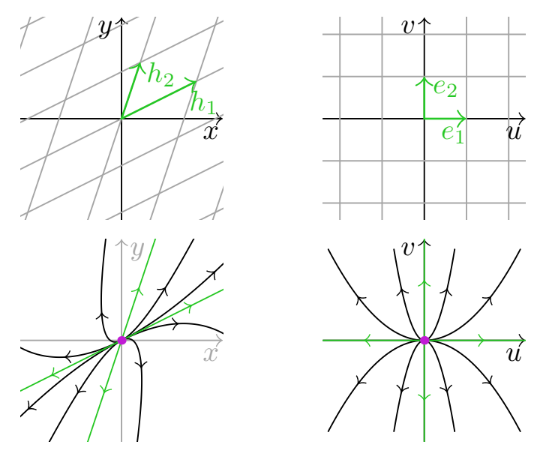
\includegraphics[scale=0.5]{Pics/neust_uzel.png}}
    \caption{Неустойчивый узел в старой и новой системе координат}
\end{figure}

При возвращении к прежней системе координат фазовый портрет исказится, но качественное поведение траекторий не изменится. Это замечание относится и ко всем последующим случаям.

Если $\lambda_2 < \lambda_1 < 0$, то уравнение фазовых траекторий не меняется, но изменяется направление движения. Теперь фазовые точки стремятся к началу координат. Соответствующее положение равновесия --- \textbf{устойчивый узел} (см. \hyperref[ustuzel]{рисунок}).

\begin{figure}[H]\label{ustuzel}
    \center{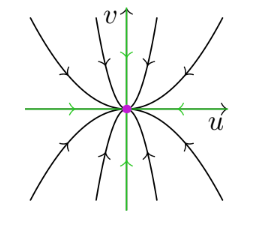
\includegraphics[scale=0.5]{Pics/ust_uzel.png}}
    \caption{Устойчивый узел}
\end{figure}

Если $\lambda_1 < 0 < \lambda_2$, то $v = Cu^{\frac{\lambda_2}{\lambda_1}}$ --- уравнение гиперболы. Соотношения $u = C_1e^{\lambda_1 t} \to 0$, $v = C_2e^{\lambda_2 t} \to \infty$ при $t \to +\infty$ дают представление о направлении движения вдоль фазовых траекторий. Точка покоя называется \textbf{седло} (см. \hyperref[sedlo]{рисунок}), она неустойчива. Асимптоты фазовых траекторий называют \textbf{сепаратрисами седла}. В старой системе координат сепаратрисы проходят вдоль собственных векторов матрицы коэффициентов.

\begin{figure}[H]\label{sedlo}
    \center{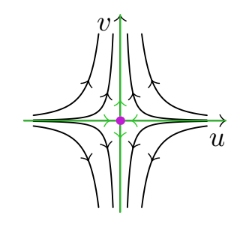
\includegraphics[scale=0.5]{Pics/sedlo.png}}
    \caption{Седло}
\end{figure}

\noindent \textbf{Случай $\lambda_1 = \lambda_2$}

Если геометрическая кратность собственного числа $\lambda = \lambda_{1,2}$ равна двум, то $A = diag(\lambda, \lambda)$. Тогда решения системы $x = C_1e^{\lambda t}$, $y = C_2e^{\lambda t}$. Исключая отсюда параметр $t$ получаем, что фазовые траектории --- лучи, входящие в начало координат при $\lambda < 0$, и выходящие из него, если $\lambda > 0$. Соответствующая точка покоя --- устойчивый или неустойчивый \textbf{дикритический узел} (см. \hyperref[dikrit]{рисунок}).

\begin{figure}[H]\label{dikrit}
    \center{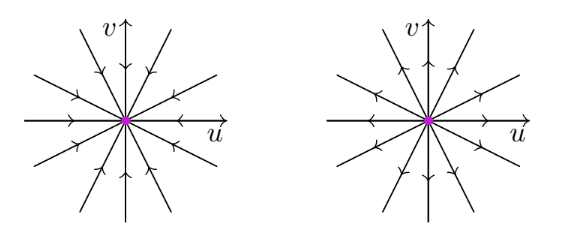
\includegraphics[scale=0.5]{Pics/dikrit.png}}
    \caption{Устойчивый и неустойчивый дикритический узел}
\end{figure}

Пусть собственное число $\lambda$ имеет геометрическую кратность $1$. Подставляя в систему $r = Ts$, где $T$ --- матрица перехода к жорданову базису, получаем
\begin{equation*}
    \dot{s} =
    \begin{pmatrix}
    \lambda & 1\\
    0 & \lambda
    \end{pmatrix}
    s
\end{equation*}
Тогда
\begin{equation*}
    s = C_1e^{\lambda t}
    \begin{pmatrix}
    1\\
    0
    \end{pmatrix}
    + C_2e^{\lambda t} (t
    \begin{pmatrix}
    1\\
    0
    \end{pmatrix}
    +
    \begin{pmatrix}
    0\\
    1
    \end{pmatrix}
    )
\end{equation*}
Следовательно, $u = C_1e^{\lambda t} + C_2te^{\lambda t}$, $v = C_2e^{\lambda t}$.

Заметим, что одновременная замена знака у постоянных $C_1$ и $C_2$ переводит фазовую траекторию в симметричную ей относительно начала координат. При $C_1 \neq 0$, $C_2 = 0$ функции $u$ и $v$ определяют полуоси координатной оси $u$. Таким образом, достаточно изучить фазовый портрет при $v > 0$.

Выражая параметр $t$ через $v$ и подставляя его в выражение для $u$, находим уравнение траекторий
\begin{equation*}
    u = Cv + \frac{\ln{v}}{\lambda}v
\end{equation*}
где $C = \frac{C_1}{C_2}$. Производная $u'_v$ указывает на то, что все фазовые траектории касаются оси $u$ при $v \to 0$ (см. \hyperref[virozhd]{рисунок}). Соответствующая точка покоя --- \textbf{вырожденный узел} (устойчивый при $\lambda < 0$ и неустойчивый при $\lambda > 0$).

\begin{figure}[H]\label{virozhd}
    \center{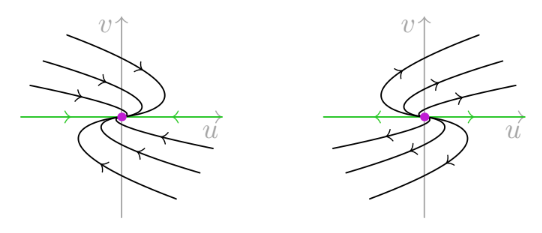
\includegraphics[scale=0.5]{Pics/virozhd.png}}
    \caption{Устойчивый и неустойчивый вырожденный узел}
\end{figure}